\section{引言}\label{sec:introduction}

知识蒸馏（KD）将教师模型的预测信息迁移给较小的学生模型。自回归语言模型蒸馏目前已涵盖替代散度、同策略训练、自适应监督和教师选择。这些进展表明，更强的教师模型并不必然产生更强的学生模型。在选择更复杂的算法之前，一个实际问题需要先得到回答：对于一个已经训练过的学生模型，冻结教师监督能否优于从完全相同的状态出发的最大似然续训？

\begin{figure}[!t]
\centering
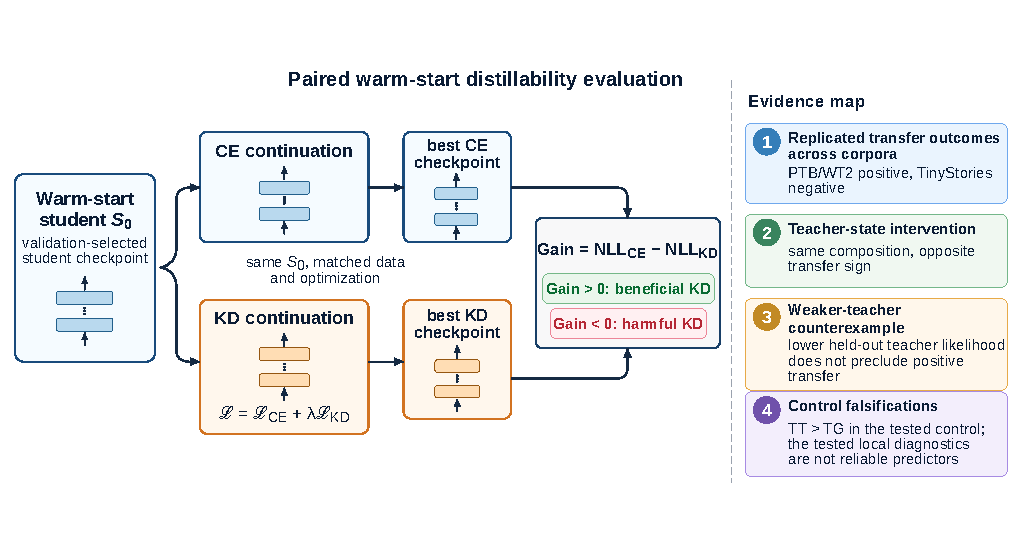
\includegraphics[width=\textwidth]{figures/fig1_paired_protocol.pdf}
\caption{配对热启动评估。完全相同的 $S_0$ 权重分别初始化 CE 和 KD；两者独立地基于验证集选择检查点，随后报告测试集结果。证据图将重复验证的迁移结果与解释范围受限的对照区分开来。}
\label{fig:paired_protocol}
\end{figure}

我们通过配对热启动评估研究这一问题。基于验证集选择的学生检查点 $S_0$ 同时初始化交叉熵（CE）续训和 KD 续训。两条实验路径均使用重新初始化的优化器，匹配续训数据和预算，然后独立地依据验证集似然选择检查点。两者的测试集 NLL 差值衡量的是在 CE 之外加入监督的价值，而不是相对于无关基线的改进。每项确认性比较均使用三个独立训练的学生初始化。

这一设计在相同的按词元归一化的 KD 形式下，揭示了可复现的正迁移和负迁移。PTB 和 WikiText-2 上的平均增益分别为 $0.1449$ 和 $0.1557$ NLL，而 TinyStories 上的性能退化幅度为 $0.1072$。每个领域的全部三个学生模型均呈现相同方向。这些结果并未确立语料身份的因果效应，因为各配置的教师模型、数据量和准备历史有所不同。因此，我们通过更受控的比较检验可能的解释。

教师质量是一项重要但不完整的解释。在固定 WikiText-2 教师架构、教师源身份和融合组成的条件下，联合训练的教师模型改善了全部三个学生模型，而仅训练融合权重的状态损害了全部三个学生模型。配对对比为 $0.1833$ NLL。教师训练状态及其产生的预测质量会明显影响迁移，但这一干预并未将标量似然单独识别为原因。相反，一个留出集似然比每个匹配的、基于验证集选择的 CE 对照都更差的 Grassmann-only 教师源，仍然改善了全部三个学生模型。因此，教师模型相对于匹配 CE 对照的似然优势并不是正迁移的必要条件。

在固定的 Transformer--Grassmann 检查点内，融合监督比任一单独分支的迁移效果更好。然而，同构 Transformer--Transformer 对照在全部三个学生模型上均取得了更好的 KD 终点，尽管其分支分歧度更低。教师质量、参数量和训练历史的差异，使我们无法将这一排序归因于架构。这一对照不支持 Grassmann 表征具有独特可迁移性，也不支持异构监督更优的主张。

回顾性的局部梯度和曲率分数也错误分类了若干在终点评估中稳定呈现正迁移的配置。我们将这些失败视为解释范围受限的证伪证据，而不是新的预测器或普遍的不可能性结论。所检验的统计量不能概括漫长的优化轨迹和基于验证集的选择。

本文的贡献是一条受控实证证据链：相对于配对 CE 对照的正迁移和负迁移、固定融合组成下的教师模型状态干预与迁移方向逆转、较弱教师源的反例、同构集成证伪对照，以及回顾性局部诊断指标的失败。我们不提出新的 KD 算法，也不声称首次发现有害 KD 或弱教师 KD。其实际意义在于，应当从所关注的学生状态出发，以匹配续训为对照评估教师监督，而不是根据单一的教师质量、多样性或局部兼容性统计量推断其价值。
